\documentclass{bredelebeamerKareem}
% \usepackage{pgf}
% \usepackage{rotating} % for defining \schwa
% \usepackage{bm}
% \usepackage{epsf}
\usepackage{graphicx}
\usepackage{algorithm}
%\usepackage{algorithmic}
\usepackage{algpseudocode}

\usepackage{cite}
% \usepackage{latexsym}
\usepackage{amssymb}
\usepackage{amsmath}
\usepackage{verbatim}
\usepackage{array}
% \usepackage{booktabs}
% \usepackage{inputenc}
\usepackage{amsthm}
\usepackage{color}
\usepackage{colortbl}
\usepackage{stmaryrd}
\usepackage{tabularx}
\usepackage{helvet}
\usepackage{multirow}
% \usepackage{placeins}
\usepackage{makecell}
% \usepackage{tablefootnote}
% \usepackage{bbding}
\usepackage{appendixnumberbeamer}
\usepackage{cleveref}
\usepackage{subcaption}
% \usepackage[nomessages]{fp}
% \usepackage[final]{pdfcomment}
\usepackage{animate}
\usepackage{multicol}
\usepackage{subfiles}
\usepackage{IEEEtrantools}
\usepackage{collcell}
\usepackage{varwidth}

\usetikzlibrary{positioning}
\usetikzlibrary{patterns}

% Place user-defined commands below.
\hyphenation{Bar-celona City-scapes auto-no-mous thril-ler beam-pattern wave-form}


\newcommand{\addpagenumber}{\begin{tikzpicture}[overlay,remember picture]
\node[anchor=east] at ([shift={(-6.5em,-6.75em)}] current page.north east) {\arabic{page}};
\end{tikzpicture}}



\DeclareMathSymbol{\widehatsym}{\mathord}{largesymbols}{"62}
\newcommand\lowerwidehatsym{%
		\text{\smash{\raisebox{-1.3ex}{%
					$\widehatsym$}}}%
}
\newcommand\fixwidehat[1]{%
		\mathchoice
		{\accentset{\displaystyle\lowerwidehatsym}{#1}}
		{\accentset{\textstyle\lowerwidehatsym}{#1}}
		{\accentset{\scriptstyle\lowerwidehatsym}{#1}}
		{\accentset{\scriptscriptstyle\lowerwidehatsym}{#1}}
}
	
\DeclareMathSymbol{\widetildesym}{\mathord}{largesymbols}{"65}
\newcommand\lowerwidetildesym{%
		\text{\smash{\raisebox{-1.3ex}{%
					$\widetildesym$}}}%
}
\newcommand\fixwidetilde[1]{%
		\mathchoice
		{\accentset{\displaystyle\lowerwidetildesym}{#1}}
		{\accentset{\textstyle\lowerwidetildesym}{#1}}
		{\accentset{\scriptstyle\lowerwidetildesym}{#1}}
		{\accentset{\scriptscriptstyle\lowerwidetildesym}{#1}}
}


\newcommand{\I}{\mathbf{I}}
\newcommand{\J}{\mathbf{J}}
\newcommand{\Jh}{\hat{\mathbf{J}}}
\newcommand{\Jt}{\hat{\mathbf{J}}_\text{total}}
\newcommand{\Jd}{\hat{\mathbf{J}}_\text{direct}}
\newcommand{\Jat}{\hat{\mathbf{J}}_\text{AT}}
\newcommand{\A}{\mathbf{A}}
\newcommand{\Ah}{\hat{\mathbf{A}}}
\newcommand{\te}{\mathbf{t}}
\newcommand{\teh}{\hat{\mathbf{t}}}


\definecolor{lightorange}{rgb}{1, 0.9, 0.8}
\definecolor{lightblue}{rgb}{0.75, 0.8, 0.9}
\definecolor{Gray}{gray}{0.9}
\definecolor{LightCyan}{rgb}{0.88,1,1}
\definecolor{DarkCyan}{rgb}{0,1,1}
\definecolor{BlueSlides}{RGB}{20,115,160}
\definecolor{Cyan}{rgb}{0.4,1,1}


\newcommand*\circled[1]{\tikz[baseline=(char.base)]{\node[shape=circle,draw,inner sep=.05pt] (char) {#1};}}

\DeclareMathOperator{\re}{Re}
\DeclareMathOperator{\im}{Im}
\DeclareMathOperator*{\argmin}{arg\,min}
\DeclareMathOperator*{\argmax}{arg\,max}
\DeclareMathOperator{\rank}{rank}
\DeclareMathOperator{\sinc}{sinc}

\makeatletter
\newcommand{\pushright}[1]{\ifmeasuring@#1\else\omit\hfill$\displaystyle#1$\fi\ignorespaces}
\newcommand{\pushleft}[1]{\ifmeasuring@#1\else\omit$\displaystyle#1$\hfill\fi\ignorespaces}
\makeatother

\newcommand{\tcb}[1]{\textcolor{blue}{#1}}
\newcommand{\tcr}[1]{\textcolor{red}{#1}}
\newcommand{\tcP}[1]{\textcolor{purple}{#1}}
\newcommand{\tcg}[1]{\textcolor{magenta}{#1}}


\Crefname{equation}{Eq.}{Eqs.}
\Crefname{figure}{Fig.}{Figs.}
% \Crefname{tabular}{Tab.}{Tabs.}

\newcolumntype{Y}{>{\centering\arraybackslash}X}
\newcolumntype{Z}{>{\raggedleft\arraybackslash}X}

\newcolumntype{L}{>{\raggedright\arraybackslash$}X<$}
\newcolumntype{M}{>{\centering\arraybackslash$}X<$}
% \newcolumntype{N}{>{\raggedleft\arraybackslash$}X<$}

\newcolumntype{A}{>{\small}l}
\newcolumntype{B}{>{\small}c}
\newcolumntype{C}{>{\small}r}
\newcolumntype{g}{>{\columncolor{Gray}}c}


\newcommand{\headline}[1]{\par\noindent\emph{\textbf{#1}}~}


\newcommand{\multiline}[2]{\begin{tabular}{@{}#1@{}}#2\end{tabular}}


\makeatletter
\providecommand{\onedot}{\futurelet\@let@token\@onedot}
\providecommand{\@onedot}{\ifx\@let@token.\else.\null\fi\xspace}
\makeatother

\providecommand{\eg}{\emph{e.g}\onedot} 
\providecommand{\Eg}{\emph{E.g}\onedot}
\providecommand{\ie}{\emph{i.e}\onedot} 
\providecommand{\Ie}{\emph{I.e}\onedot}
\providecommand{\cf}{\emph{c.f}\onedot} 
\providecommand{\Cf}{\emph{C.f}\onedot}
\providecommand{\etc}{\emph{etc}\onedot} 
\providecommand{\vs}{\emph{vs}\onedot}
\providecommand{\wrt}{w.r.t\onedot} 
\providecommand{\dof}{d.o.f\onedot}
\providecommand{\etal}{\textit{et al}\onedot}


\newcommand{\tfn}[1]{\footnote{\tiny #1}}
\newcommand\blfootnote[1]{%
  \begingroup%
%   \setlength{\footnotesep}{1pt}%
%   \setlength{\footskip}{1pt}%
%   \setlength{\bottommargin}{1pt}%
  \renewcommand\thefootnote{}\footnote{#1}%
  \addtocounter{footnote}{-1}%
%   \restoregeometry%
  \endgroup
}


\def\yb{{\mathbf{y}}}
\def\mb{\mathbf}
\def\mc{\mathcal}
\newcommand{\norm}[1]{\lVert #1 \rVert}


\def\mb{\mathbf}
\def\bs{\boldsymbol}
\def\ds{\displaystyle}
\def\tb{\textbf}
\def\ti{\textit}



% fled
\newcommand{\desired}{\mathbf{d}}
\newcommand{\xb}{{\mathbf{x}}}
\newcommand{\xkj}{{\mathbf{x}_\kappa^{(j)}}}
\newcommand{\xoj}{{\mathbf{x}_0^{(j)}}}
\newcommand{\xij}{{\mathbf{x}_i^{(j)}}}
\newcommand{\xionej}{{\mathbf{x}_{i+1}^{(j)}}}
\newcommand{\ximj}{{\mathbf{x}_{i-1}^{(j)}}}
\newcommand{\xijtilde}{{\mathbf{\tilde{x}}_i^{(j)}}}
\newcommand{\xijbar}{{\mathbf{\overline{x}}_i^{(j)}}}
\newcommand{\xijhat}{{\mathbf{\hat{x}}_i^{(j)}}}
\newcommand{\etaij}{{\boldsymbol{\eta}_{i}^{(j)}}}
\newcommand{\etaijbar}{{\overline{\boldsymbol{\eta}}_{i}^{(j)}}}



% slides related
\newcommand{\pdfnote}[1]{\marginnote{\pdfcomment[icon=note]{#1}}}



% defect

%The min, mid and max values
\newcommand*{\MinNumber}{0.0}%
\newcommand*{\MidNumber}{0.5}%
\newcommand*{\MaxNumber}{1.0}%
%Apply the gradient macro
\newcommand{\ApplyGradient}[1]{%
        \ifdim #1 pt > \MidNumber pt
            \pgfmathsetmacro{\PercentColor}{max(min(100.0*(#1 - \MidNumber)/(\MaxNumber-\MidNumber),100.0),0.00)} %
            \hspace{-0.33em}\colorbox{BlueSlides!\PercentColor!lightblue}{$\mathbf{#1}$}
        \else
            \pgfmathsetmacro{\PercentColor}{max(min(100.0*(\MidNumber - #1)/(\MidNumber-\MinNumber),100.0),0.00)} %
            \hspace{-0.33em}\colorbox{white!\PercentColor!lightblue}{$\mathbf{#1}$}
        \fi
}

\newcolumntype{R}{>{\collectcell\ApplyGradient}c<{\endcollectcell}}

\newcommand{\startconfmat}{%
\renewcommand{\arraystretch}{0}%
\setlength{\fboxsep}{3mm} % box size
\setlength{\tabcolsep}{0pt}%
}
\newcommand{\wrapconfmat}{%
\renewcommand{\arraystretch}{1}%
\setlength{\tabcolsep}{3pt}%
}

\makeatletter
\newcommand{\confmatone}[5]{
\begin{subtable}{0.38\linewidth}
\def\inp{#1}
\centering\ifx\inp\@empty\else\caption{\scriptsize #1}\fi
\begin{tabular}{ccRR}
\ifx\inp\@empty\else%
&  & \multicolumn{2}{c}{Prediction}\\[0.5em]
&  & \multicolumn{1}{c}{$(-)$} & \multicolumn{1}{c}{$(+)$}\\[0.5em]\fi
\multirow{2}{5mm}{\rotatebox[origin=c]{90}{Label}} & \parbox[t]{5mm}{\rotatebox[origin=c]{90}{$(-)$}} & #2 & #3 \\
% \multirow{2}{*}{\parbox[b]{4mm}{\rotatebox[origin=c]{90}{ True Label}}} & \multicolumn{1}{c}{\parbox[t]{4mm}{\rotatebox[origin=c]{90}{$(-)$}}} & #2 & #3 \\
 & \parbox[t]{5mm}{\rotatebox[origin=c]{90}{$(+)$}} & #4 & #5 \\
\end{tabular}
\end{subtable}
}
\newcommand{\confmattwo}[5]{
\begin{subtable}{0.29\linewidth}
\def\inp{#1}
\centering\ifx\inp\@empty\else\caption{\scriptsize #1}\fi
\begin{tabular}{RR}
\ifx\inp\@empty\else%
\multicolumn{2}{c}{Prediction}\\[0.5em]
\multicolumn{1}{c}{$(-)$} & \multicolumn{1}{c}{$(+)$}\\[0.5em]\fi
#2 & #3 \\
#4 & #5 \\
\end{tabular}
\end{subtable}
}
\makeatother



\newcommand{\showbrace}[4]{{\onslide*<-#1>{#3}\onslide*<#2->{\underbrace{#3}_\text{#4}}}}

\newcommand{\modelFrameComplete}{%
\begin{frame}{FLED -- Fast, Learned and Efficient Deep Radar Beampattern Design}
\begin{canvas}
\only<2>{\node[anchor=north west] at ([shift={(0,-0.625)}] UL) {\includegraphics[width=0.99\linewidth]{fled/fled-below_only.drawio.pdf}};}
\node[anchor=north west] at (UL) {\includegraphics[width=0.99\paperwidth]{fled/fled-nobelow.drawio.pdf}};
\only<3>{\node[anchor=north] at (CC) {\includegraphics[width=0.8\linewidth]{fled/expand.drawio.pdf}};}
\end{canvas}
\end{frame}}

\newcommand{\modelFrame}[1]{%
\begin{frame}{FLED -- Fast, Learned and Efficient Deep Radar Beampattern Design}
\begin{canvas}
\node[anchor=north west] at (UL) {\includegraphics[width=0.99\paperwidth]{fled/fled-nobelow.drawio.pdf}};
\node[anchor=north] at (CC) {\begin{minipage}{\textwidth}
#1
\end{minipage}};
\end{canvas}
\end{frame}}



\newcommand{\networkSection}[1]{%
\begin{frame}{}
\centering \includegraphics[width=\linewidth]{dehazing/#1.pdf}%
\end{frame}
}



\graphicspath{{./figs/}}



\title[Explainable, Informed Deep Learning for Signal and Image Estimation]{Explainable, Informed Deep Learning \texorpdfstring{\\\smallskip}{}for Signal and Image Estimation}
\subtitle{Ph.D. Dissertation Defense}
\author[Kareem Metwaly]{Kareem Metwaly}
\advisor{Prof. Vishal Monga}
\institute[Penn State]{
Information Processing \& Algorithm Laboratory\\
The school of Electrical Engineering and Computer Science\\
The Pennsylvania State University}
\date{October $10^\text{th}, 2022$}
\subject{Ph.D. Dissertation Defense}

\setbeamerfont{author}{size=\large}

%%%%%%%%%%%%%%%%%%%%%%%%%%%%%%%%%%%%%%%%%%%%%%%%%%%

\begin{document}

% \shorthandoff{:}

\begin{frame}[plain,noframenumbering,image=0.6]
  \titlepage
\end{frame}


\begin{frame}{Outline}
  \tableofcontents[subsectionstyle=show/show/hide,]
  % option [pausesections]
\end{frame}



\section{Introduction}

\subsection{Motivation}
% deep learning vs. model based, then what we are doing


\begin{frame}{Analysis and Synthesis Problems}
\begin{tikzpicture}[overlay,remember picture,shift=(current page.south west)]
\only<1>{\node[anchor=south west] at (0,0) {\begin{animateinline}[autoplay,width=\paperwidth,poster=first,every=2]{30}\multiframe{5}{idx=1+1}{\includegraphics[width=\paperwidth]{animations/est_prob_3/est_prob-000\idx}}\end{animateinline}};}

\only<2>{\node[anchor=south west] at (0,0) {\begin{animateinline}[autoplay,width=\paperwidth,poster=first,every=2]{30}\multiframe{5}{idx=5+1}{\includegraphics[width=\paperwidth]{animations/est_prob_3/est_prob-000\idx}}\newframe\multiframe{16}{idx=10+1}{\includegraphics[width=\paperwidth]{animations/est_prob_3/est_prob-00\idx}}\end{animateinline}};}

\only<3>{\node[anchor=south west] at (0,0) {\begin{animateinline}[autoplay,width=\paperwidth,poster=first,every=2]{30}\multiframe{42}{idx=25+1}{\includegraphics[width=\paperwidth]{animations/est_prob_3/est_prob-00\idx}}\end{animateinline}};}

\only<4>{\node[anchor=south west] at (0,0) {\begin{animateinline}[autoplay,width=\paperwidth,poster=first,every=2]{30}\multiframe{25}{idx=66+1}{\includegraphics[width=\paperwidth]{animations/est_prob_3/est_prob-00\idx}}\end{animateinline}};}

\only<5>{\node[anchor=south west] at (0,0) {\begin{animateinline}[autoplay,width=\paperwidth,poster=first,every=2]{30}\multiframe{10}{idx=90+1}{\includegraphics[width=\paperwidth]{animations/est_prob_3/est_prob-00\idx}}\newframe\multiframe{31}{idx=100+1}{\includegraphics[width=\paperwidth]{animations/est_prob_3/est_prob-0\idx}}\end{animateinline}};}

\only<6>{\node[anchor=south west] at (0,0) {\begin{animateinline}[autoplay,width=\paperwidth,poster=first,every=2]{30}\multiframe{16}{idx=130+1}{\includegraphics[width=\paperwidth]{animations/est_prob_3/est_prob-0\idx}}\end{animateinline}};}
\end{tikzpicture}
\end{frame}



\titleFrame{Part}{I}{Explainable Informed Deep Learning \\\smallskip for Image Analysis}{
\begin{itemize}
\item Global, Local and Intrinsic Dense Embedding Network for \textbf{Multi-Category Attributes Prediction}.
\medskip
\item Surface \textbf{Defect Detection} and Evaluation for Marine Vessels.
\end{itemize}
}


\section[I: GlideNet]{Contribution I: Global, Local and Intrinsic Dense Embedding Network for Multi-Category Attributes Prediction}

\titleFrame{Contribution}{I}{Global, Local and Intrinsic Dense Embedding Network \\\medskip for Multi-Category Attributes Prediction}{
\begin{itemize}
\item {\small {\bf Kareem Metwaly}, Aerin Kim, Elliot Branson and Vishal Monga, “GlideNet: Global, Local and Intrinsic based Dense Embedding NETwork for Multi-category Attributes Prediction,” {\em the IEEE/CVF Computer Vision and Pattern Recognition (CVPR)}, acceptance rate $25\%$, New Orleans, Louisiana, 2022.}
\medskip
\item {\small {\bf Kareem Metwaly}, Aerin Kim, Elliot Branson and Vishal Monga, “CAR – Cityscapes Attributes Recognition A Multi-category Attributes Dataset for Autonomous Vehicles,” to be submitted, arXiv:2111.08243.}
\end{itemize}
}


\subsection{GlideNet}


\begin{frame}{GlideNet Architecture}
\begin{figure}
\foreach \n [count=\y] in {0,...,3,0,0}{\only<\y>{\includegraphics[width=\linewidth]{glidenet/network_\n.pdf}}}
    \caption{GlideNet Architecture}
\end{figure}

\onslide<6>{
\begin{itemize}  
\item Training this complex architecture is divided into two stages:\smallskip
	\begin{itemize}
  	    \item Stage I: training each feature extractor independently (GFE, LFE \& IFE). \note{The focus here is to make sure that each feature extractor is actually generating the features related to its objective. For instance, GFE should generate features that helps in understanding the whole scene not just the object of interest.}
	    \smallskip
	    \item Stage II: estimating the attributes. \note{This is similar to the actual inference step. The decoders used to guide training in stage I are removed (except for category estimation module). Then the main focus is in estimating the final attributes vector to be as close as possible to the groundtruth.}
	\end{itemize}
\end{itemize}}
\end{frame}


\begin{frame}{Training -- Feature Extractors -- GFE}
\begin{tikzpicture}[overlay,remember picture]
\node[anchor=north] (PIC) at ([yshift={-6em}] current page.north) {\includegraphics[width=\framewidth]{glidenet/gfe_training}};
\node[below,anchor=north] at ([yshift={-10em}] PIC) {\resizebox{\linewidth}{!}{$\mathcal{L}_\text{g} = \lambda_{gp0}\showbrace{1}{2}{\mathcal{L}_\text{BCE}\left( P_0, \hat{P_0}\right)}{confidence} + \lambda_{gp}\showbrace{2}{3}{\mathcal{L}_\text{CE}\left(\textbf{P}, \hat{\textbf{P}}\right)}{Prob. Dist.} + \lambda_{gd}\showbrace{3}{4}{\left[\mathcal{L}_\text{MSE}\left(H,\hat{H}\right) + \mathcal{L}_\text{MSE}\left(W,\hat{W}\right)\right]}{size of the bounding box} + \lambda_{gc}\showbrace{4}{5}{\left[\mathcal{L}_\text{MSE}\left(C_x, \hat{C}_x\right) + \mathcal{L}_\text{MSE}\left(C_y, \hat{C}_y\right)\right]}{center coordinates of the bounding box}$}};
\end{tikzpicture}
\end{frame}




\section[II: Defect Detection]{Contribution II: Surface Defect Detection and Evaluation for Marine Vessels}

\titleFrame{Contribution}{II}{Surface Defect Detection and Evaluation for Marine Vessels}{
\begin{itemize}
\item {\small Li Yu*, {\bf Kareem Metwaly}*, James Wang and Vishal Monga, “Surface Defect Detection and Evaluation for Marine Vessels using Multi-Stage Deep Learning,” {\em IEEE transactions on Intelligent Transportation Systems} (IEEE T-ITS). *Equal Contribution, under review (revision to be submitted October 2022), arXiv:2203.09580.}
\end{itemize}
}


\subsection{Proposed Model}


\begin{frame}{Proposed Pipeline}
\begin{tikzpicture}[overlay,remember picture]
\node[anchor=center] at (current page.center) {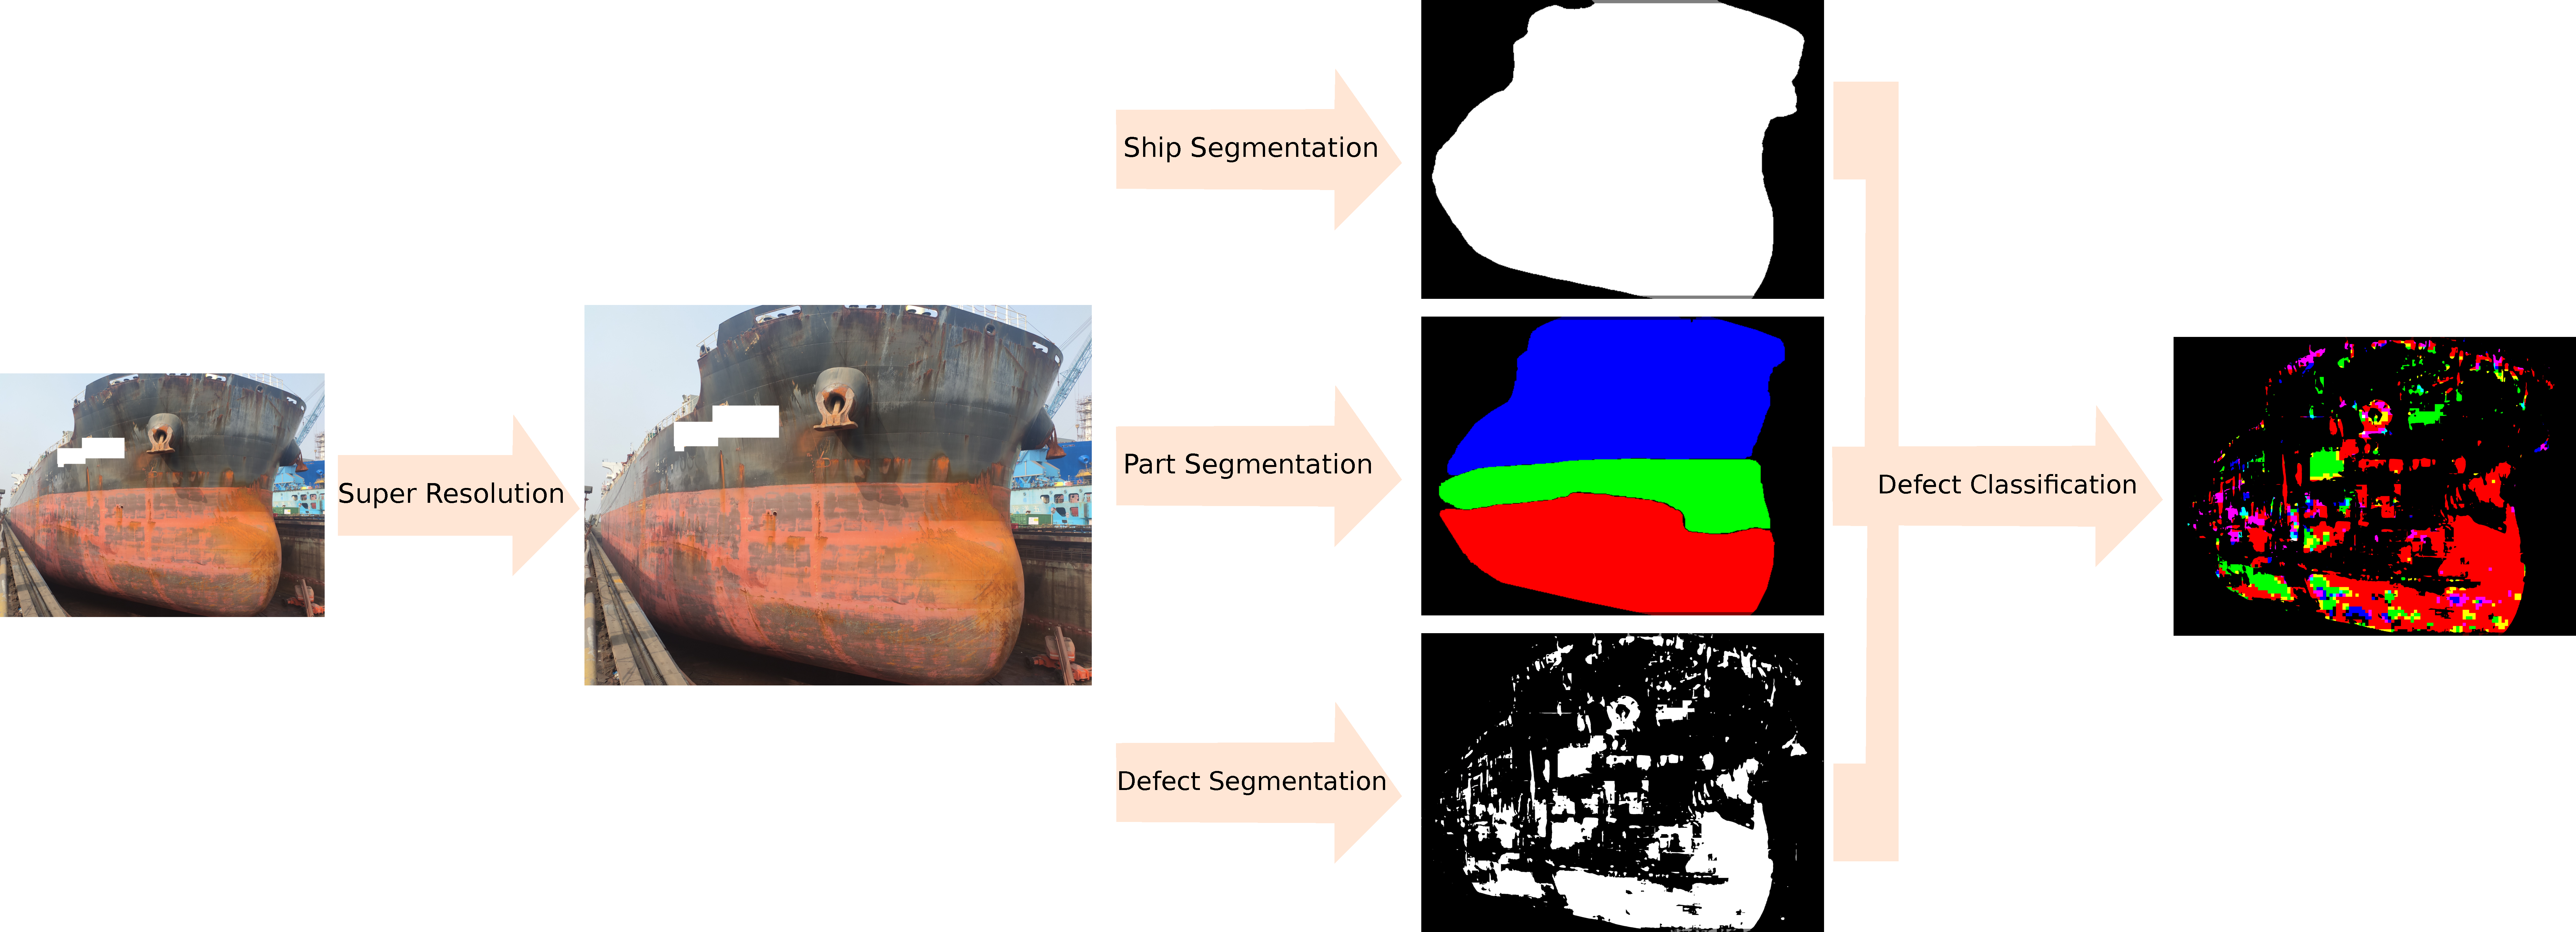
\includegraphics[width=\textwidth]{defect/pipeline_horizontal_compressed.pdf}
};
\onslide<1>{\draw[draw=none, fill=white, fill opacity=0.9] ([shift={(80pt, -50pt)}] current page.north west) rectangle (current page.south east);}
\onslide<2>{\draw[draw=none, fill=white, fill opacity=0.9] ([shift={(200pt, -50pt)}] current page.north west) rectangle (current page.south east);}
\onslide<3>{\draw[draw=none, fill=white, fill opacity=0.9] ([shift={(311pt, -50pt)}] current page.north west) rectangle (current page.south east);}
\onslide<4>{};
\end{tikzpicture}
\end{frame}


\begin{frame}{DFE-NET}
\begin{tikzpicture}[overlay,remember picture]
\only<2>{\node[anchor=north] at ([shift={(-5em,-5em)}] NET) {\includegraphics[width=0.7\textwidth]{defect/stn.pdf}};}
\only<3>{\node[anchor=south] at ([yshift={2em}] current page.south) {\begin{varwidth}{\linewidth}\begin{align}
            \mathcal{L} &= \sum_{i=1}^3 w_i \mathcal{L}_\text{BCE}^{(i)}(l_i, p_i) + \lambda \cdot \left|\text{CosSim}\left(F_G, F_D\right)\right| \\
            \mathcal{L}_\text{BCE}^{(i)}(l_i, p_i) &= l_i \log{p_i} + (1 - l_i) \log(1 - p_i) \\
            \text{CosSim}\left(x, y\right) &= \frac{x^T y}{\max\left(||x||\cdot ||y||, \epsilon\right)}
\end{align}\end{varwidth}};}
\node[anchor=north] (NET) at ([yshift={(-5em)}] current page.north) {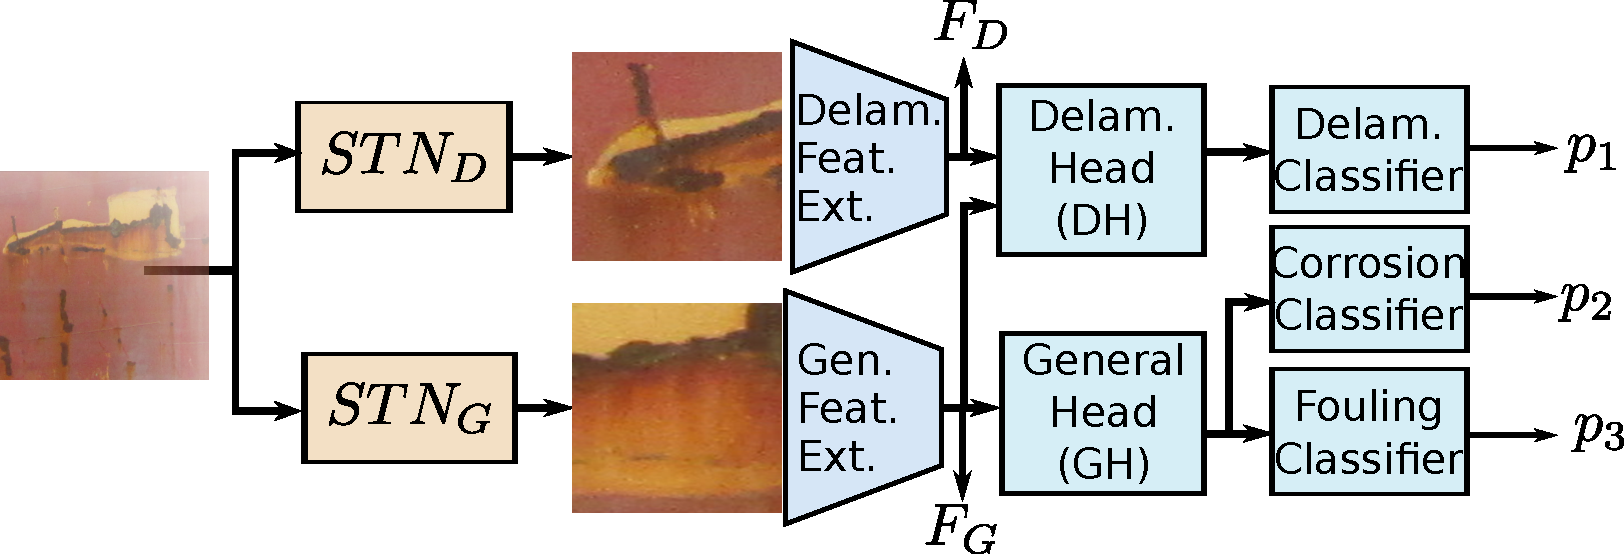
\includegraphics[width=0.95\textwidth]{defect/arch_nostn.pdf}};
\end{tikzpicture}
\footnotetext[1]{STN is based on Jaderberg \etal, ``Spatial Transformer Networks,'' {\em NeurIPS}, 2017}
\end{frame}


\subsection{Pipeline Results}

\startconfmat

\begin{frame}{Confusion Matrices of Different Defect Types}
\hfill\begin{minipage}{0.15\linewidth}
\vspace{3em}
Corrosion\\[6em]
\onslide<2->{Delamination}\\[6em]
\onslide<3->{Fouling}
\end{minipage}%
\begin{minipage}{0.85\linewidth}
\begin{minipage}{\linewidth}
\hspace{6.5em} without DFE \hspace{6em} DFE without regul. \hspace{5em} DFE with regul.
\end{minipage}\\[1em]
\begin{minipage}{\linewidth}
\hspace{7em} Prediction \hspace{8.5em} Prediction \hspace{8em}Prediction
\end{minipage}\\
\begin{minipage}{\linewidth}
\hspace{6.5em} $(-)\,\,\qquad(+)$ \hspace{7em} $(-)\,\,\qquad(+)$ \hspace{7em}$(-)\,\,\qquad(+)$
\end{minipage}\\
\begin{minipage}{\linewidth}
\begin{table}
\centering

\confmatone{}{0.85}{0.15}{0.28}{0.72}\hfill
\confmattwo{}{0.85}{0.15}{0.23}{0.73}\hfill
\confmattwo{}{0.87}{0.13}{0.24}{0.76}

\vspace{1em}

\onslide<2->{
\confmatone{}{0.68}{0.32}{0.53}{0.47}\hfill
\confmattwo{}{0.72}{0.28}{0.47}{0.53}\hfill
\confmattwo{}{0.75}{0.25}{0.46}{0.54}
}

\vspace{1em}

\onslide<3->{
\confmatone{}{0.72}{0.28}{0.24}{0.76}\hfill
\confmattwo{}{0.76}{0.24}{0.20}{0.80}\hfill
\confmattwo{}{0.77}{0.23}{0.18}{0.82}
}
\end{table}
\end{minipage}
\end{minipage}
\end{frame}

\wrapconfmat




\titleFrame{Part}{II}{Explainable Informed Deep Learning \\\medskip for Image and Signal Synthesis}{
\begin{itemize}
\item NonLocal Channel Attention for NonHomogeneous \textbf{Image Dehazing}.
\medskip
\item Fast, Learned and Explainable Deep Radar \textbf{Beampattern Design}.
\end{itemize}
}


\section[III: Dehazing]{Contribution III: NonHomogeneous Haze Removal}

\titleFrame{Contribution}{III}{NonLocal Channel Attention \\\medskip for NonHomogeneous Image Dehazing}{
\begin{itemize}
\item {\small {\bf Kareem Metwaly}, Xuelu Li, Tiantong Guo and Vishal Monga, ``NonLocal Channel Attention for NonHomogeneous Image Dehazing,'' {\em the IEEE/CVF Computer Vision and Pattern Recognition (CVPR)} workshops, {\bf runner-up} in SSIM metric, Seattle, Washington, 2020.}
\medskip
\item {\small Co-author of Codruta O. Ancuti, et al. ``NTIRE 2020 Challenge on NonHomogeneous Dehazing,'' {\em The IEEE/CVF Conference on Computer Vision and Pattern Recognition (CVPR)} Workshops, 2020, pp. 490-491.}
\end{itemize}
}



\subsection{Proposed Method: AtJwD}


\multipleframe
\networkSection{network}
\subframe\networkSection{top}
\subframe\networkSection{enc}
\subframe\networkSection{physical}
\subframe\networkSection{direct}
\subframe\networkSection{weight}
\subframe\networkSection{dec}
\subframe\networkSection{dilation}
\subframe\networkSection{se}
\subframe\begin{frame}{}
\centering 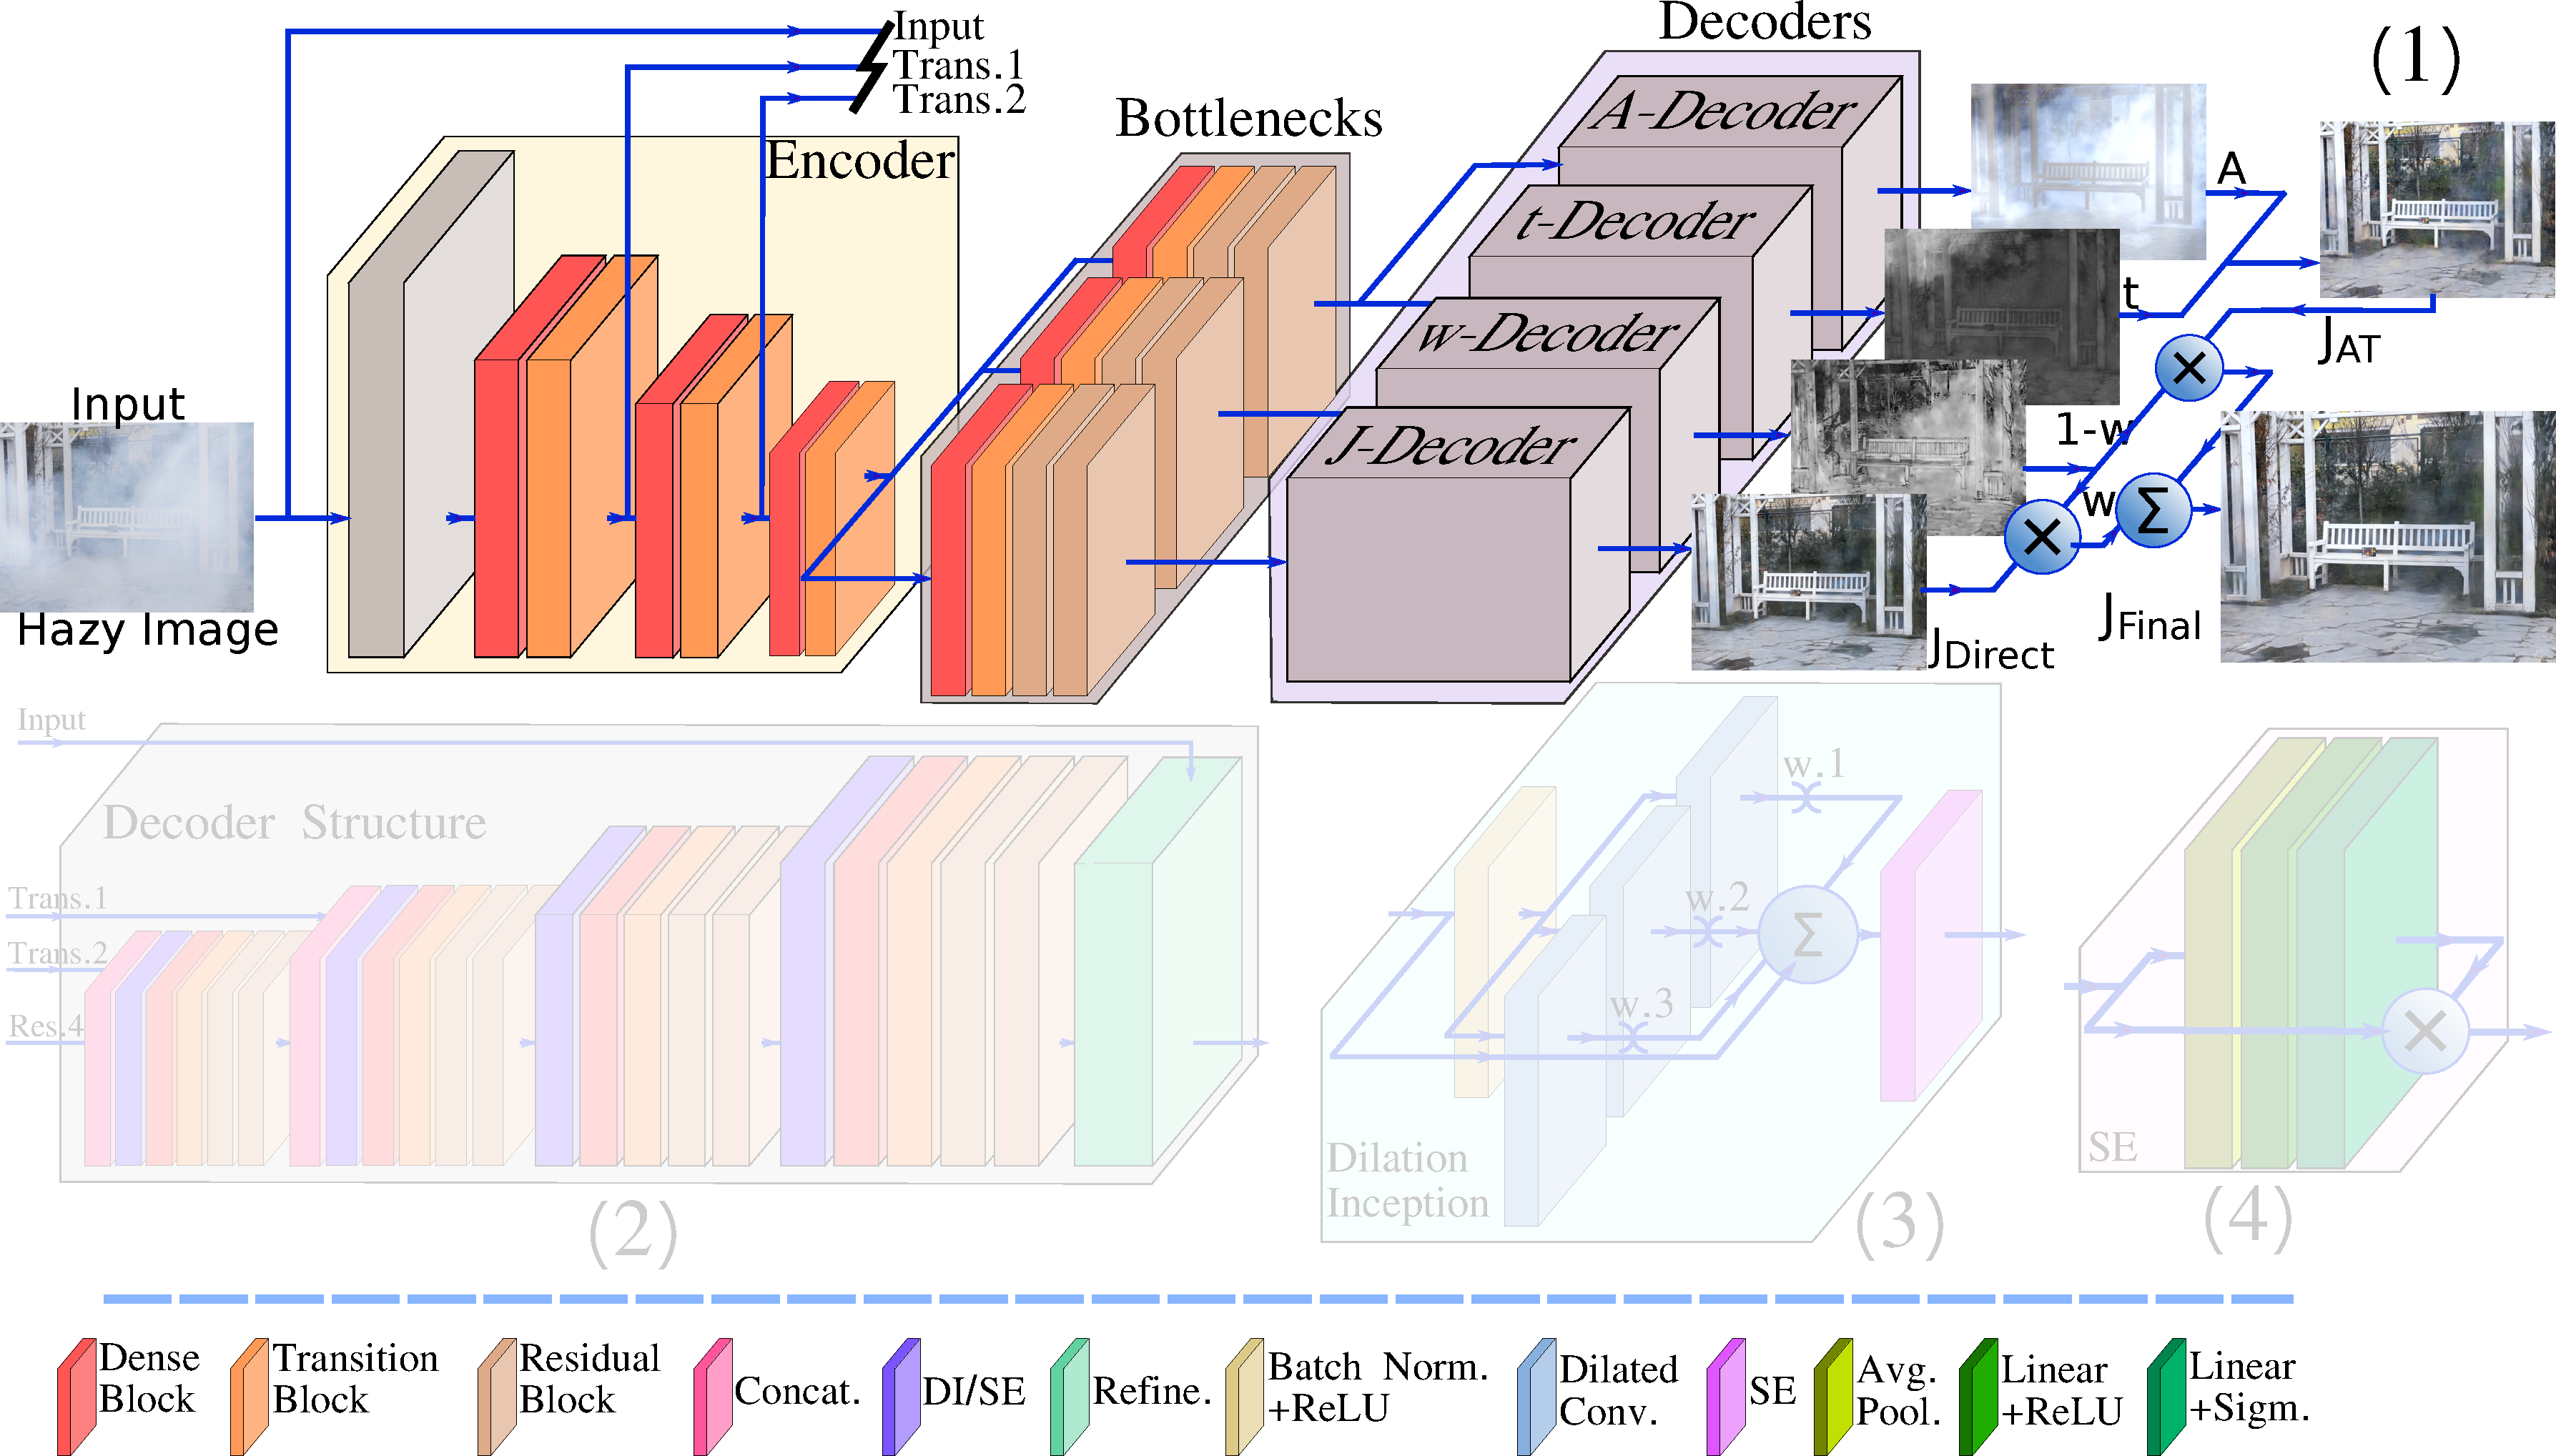
\includegraphics[width=\linewidth]{dehazing/top.pdf}%
\begin{canvas}
\draw[draw=none,fill=white,opacity=0.8] (-1,-0.0625) rectangle (1,-0.75);
\node[anchor=north] at (current page.center) {\begin{varwidth}{\linewidth}\begin{align}
\mathcal{L} &= \mathcal{L}_{rec}+\lambda_p\mathcal{L}_p+\lambda_s\mathcal{L}_s+\lambda_A\mathcal{L}_\text{var}\\
\tcb{\text{Reconstruction Term} \rightarrow}\quad\mathcal{L}_{rec} &= \|\Jt - \J\|_2^2 + \lambda_c \left(\|\Jd - \J\|_2^2 + \|\Jat - \J\|_2^2\right)\\
\tcb{\text{Perceptual Term} \rightarrow}\quad\mathcal{L}_p &= \|G(\Jt) - G(\J)\|_2^2\\
\tcb{\text{Similarity Term} \rightarrow}\quad\mathcal{L}_s &= 1 - \textbf{SSIM}(\Jt, \J)\\
\tcb{\text{Variance Term} \rightarrow}\quad\mathcal{L}_\text{var} &= \sigma_A^2
\end{align}\end{varwidth}};
\end{canvas}
\end{frame}
\subframe\networkSection{network}
\restoreframe



\section[IV: FLED]{Contribution IV: Fast, Learned and Explainable Deep Radar Beampattern Design}

\titleFrame{Contribution}{IV}{Fast, Learned and Explainable Deep Radar Beampattern Design}{
\begin{itemize}
\item {\small {\bf Kareem Metwaly}, Junho Kweon, Khaled Alhujaili, Maria S. Greco, Fulvio Gini and Vishal Monga, ``Interpretable, Unrolled Deep Radar Beampattern Design,'' {\em the IEEE International Conference on Acoustics, Speech, and Signal Processing
 (ICASSP) 2023}, submitted.}
\item {\small {\bf Kareem Metwaly}, Junho Kweon, Khaled Alhujaili, Maria S. Greco, Fulvio Gini and Vishal Monga, ``Fast, Learned and Explainable Deep Radar Beampattern Design,'' {\em the IEEE Transactions on Signal Processing (TSP)}, in preparation.}
\end{itemize}
}



\begin{frame}{What is Algorithm Unrolling? and Why?}
\begin{canvas}
\def\figheight{0.9\textheight}
\def\skipfreq{8}
\def\playspeed{100}
\only<1>{\node[anchor=center] at (CC) {\animategraphics[autoplay,height=\figheight,poster=first,every=\skipfreq]{\playspeed}{animations/plot3d/im-}{10}{199}};}
\only<2>{\node[anchor=center] at (CC) {
\begin{animateinline}[autoplay,height=\figheight,poster=first,every=\skipfreq]{\playspeed}
\multiframe{108}{idx=199+-1}{\includegraphics[height=\figheight]{animations/plot3d/im-\idx}}
\newframe
\multiframe{109}{idx=0+1}{\includegraphics[height=\figheight]{animations/plot3d/rotate/im-\idx}}
\newframe
\multiframe{\skipfreq}{}{\includegraphics[height=\figheight]{animations/plot3d/rotate/im-108.png}}
\end{animateinline}};}
\only<3-6>{\node[anchor=center] at (CC) {\includegraphics[height=\figheight]{animations/plot3d/rotate/im-108.png}};}


\node (GO) at (0.0469,-5/16) {};
\node (LO) at (0.25,0.0938) {};
\node (PEAK) at (0.1562,1/2) {};
\node (XBAD) at (0.375,0.3125) {};
\node (XGOOD) at (0.0938,0) {};

\only<3-6>{
\draw[anchor=center,draw=red,thick] (GO) circle (3mm and 2mm);
\node (GOT) at ([shift=({-1/4,-1/4})] GO) {\tcr{Global Minimum}};
\draw[red,->] (GOT) -- (GO);
}
\only<4-6>{
\draw[anchor=center,draw=blue,thick] (LO) circle (3mm and 2mm);
\node (LOT) at ([shift=({1/4,-1/4})] LO) {\tcb{Local Minimum}};
\draw[blue,->] (LOT) -- (LO);
}
\only<5-6>{
\draw[anchor=center,draw=blue,thick,fill=Black] (XBAD) circle (1mm);
\node (XB) at ([shift=({1/32,1/32})] XBAD) {$X_1$};
\draw[anchor=center,draw=blue,thick,fill=Black] (XGOOD) circle (1mm);
\node (XG) at ([shift=({-1/32,1/32})] XGOOD) {$X_2$};
}
\only<6>{
\draw[->,ultra thick,magenta] (0.125,0.125) -- (0.0624,-0.125); %Good
\draw[->,ultra thick,magenta] (0.4375,0.3438) -- (0.3125,0.2812); %Bad
}

\only<7>{\node[anchor=center] at (CC) {
\begin{animateinline}[autoplay,height=\figheight,poster=first,every=\skipfreq]{60}
\multiframe{109}{idx=108+-1}{\includegraphics[height=\figheight]{animations/plot3d/rotate/im-\idx}}
\newframe
\multiframe{108}{idx=90+1}{\includegraphics[height=\figheight]{animations/plot3d/im-\idx}}
\newframe
\multiframe{31}{idx=0+1}{\includegraphics[height=\figheight]{animations/plot3d/rotate_all/im-\idx}}
\multiframe{\skipfreq}{}{\includegraphics[height=\figheight]{animations/plot3d/rotate_all/im-30.png}}
\newframe\multiframe{1}{}{\includegraphics[height=\figheight]{animations/plot3d/rotate_all/im-30.png}}
\end{animateinline}};}

\only<8->{\node[anchor=center] at (CC) {\includegraphics[height=\figheight]{animations/plot3d/rotate_all/im-30.png}};}

\node (AU) at (1/16,-1/16) {};
\node (IA) at (-1/8,1/4) {};
\node (DL) at (1/8,-1/4) {};

\only<8->{
\draw[pattern=north west lines,magenta,opacity=0.5,draw=none] (IA) circle (3mm);
\node[above=3mm,magenta] at (IA) {\large \bf Iterative Algorithms};
}
\only<9->{
\draw[pattern=north west lines,orange,opacity=0.5,draw=none] (DL) circle (14mm);
\node[below=14mm,orange] at (DL) {\large \bf Deep Learning};
}
\only<10->{
\draw[pattern=north west lines,red,opacity=0.4] (AU) circle (3mm);
\node[above=3mm,red] at (AU) {\large \bf Algorithm Unrolling};
}
\end{canvas}
\end{frame}


\begin{frame}{PDR: Iterative Algorithm}
\begin{minipage}[c]{.55\linewidth}
\small
\quad\textbf{Algorithm:}Projection-Descent-Retraction (PDR)
\begin{algorithmic}
	\State \resizebox{\linewidth}{!}{\textbf{Inputs: } $\bar{f}(\mathbf x)$, $\mathbf x_{(0)} \in \mathcal{S}^L$, $\beta$ and a pre-defined threshold value $\epsilon$.}
	\State \textbf{Output: } A solution $\mathbf x^{\star}$ for optimizing $\bar{f}(\mathbf x)$ over $\mathcal{S}^L$.
	\State (1) Set $k=0$.
	\State (2) Evaluate the search direction: $\boldsymbol{\eta}_{(k)}=-\nabla_{\mathbf x} \bar{f}(\mathbf x_{(k)})$.
	\State (3) Compute the projection of the $\boldsymbol{\eta}_{(k)}$ onto the tangent space  
	$$\mathbf{P}_{\mathcal{T}_{\mathbf x_{(k)}}\mathcal{S}^L}\big(\boldsymbol{\eta}_{(k)}\big)=\boldsymbol{\eta}_{(k)} - \text{Re}\{\boldsymbol{\eta}_{(k)}^{*}\odot \mathbf x_{(k)}\}\odot \mathbf x_{(k)}$$ 
	\State (4) Update $\mathbf x_{(k)}$ on $\mathcal{T}_{\mathbf x_{(k)}}\mathcal{S}^L$: $$\bar{\mathbf{x}}_{(k)}=\mathbf{x}_{(k)} +\beta \mathbf{P}_{\mathcal{T}_{\mathbf x_{(k)}}\mathcal{S}^L}\big(\boldsymbol{\eta}_{(k)}\big)$$
	\State (5) Retract $\bar{\mathbf{x}}_{(k)}$ to the complex circle manifold by: 
	$$\mathbf{x}_{(k+1)}=\mathbf{R}\big(\bar{\mathbf{x}}_{(k)}\big)=\bar{\mathbf{x}}_{(k)}\odot \frac{1}{\left|\bar{\mathbf{x}}_{(k)}\right|}$$
    \If {$|\bar{f}(\mathbf{x}_{(k+1)})-\bar{f}(\mathbf{x}_{(k)})|< \epsilon$} STOP.
	\Else \quad k = k+1 and GOTO step (2).
	\EndIf
	\State \textbf{Output:} $\mathbf x^{\star}= \mathbf x_{(k+1)}$
\end{algorithmic}
\end{minipage}\hfill%
\begin{canvas}[]
\node (CircleCenter) at (0.5,-0.25) {};
\node (point) at (0.275,-0.06125) {};
\node (startTangent) at (0.196,-0.375) {};
\node (endGrad) at (0.31,0.5) {};
\node (endProject) at (0.405,0.44) {};
\node (betaStep) at (0.355,0.25) {};
\node (newPoint) at (0.385,0.145) {};


\only<2->{
\draw[<->,very thin] (CircleCenter) ++(-0.45,0) -- +(0.9,0);
\draw[<->,very thin] (CircleCenter) ++(0,-0.6) -- +(0,1.2);
\node[below] at ($(CircleCenter)+(0.45,0)$) {Re};
\node[right] at ($(CircleCenter)+(0,0.6)$) {Im};
\node at (0.75,-0.625) {\huge $\mathcal{S}^L$};
\draw[draw=black,fill=none] (CircleCenter) circle [radius=2cm];
}
\only<3->{
\draw[fill=blue] (point) circle[radius=0.5mm];
\node[below right] at (point) {$\tcb{\mathbf{x}_{(k)}}$};
}
\only<4->{
\draw[solid] (startTangent) -- (0.42,0.5);
\node[below left] at (startTangent) {$\mathcal{T}_{\mathbf x_{(k)}}\mathcal{S}^L$};
}
\only<5->{
\draw[red] (-0.8438,0.36) rectangle (-0.0938,0.2812);
\draw[->,red,thick] (point) -- (endGrad);
\node[above] at (endGrad) {\tcr{$\boldsymbol{\eta}_{(k)}$}};
}
\only<6->{
\draw[blue] (-0.8438,0.28) rectangle (0,0.0312);
\draw[dotted,thick,black] (endGrad) -- (endProject);
\draw[->,blue,thick] (point) -- (endProject);
\node[above right] at (endProject) {\tcb{$\mathbf{P}_{\mathcal{T}_{\mathbf x_{(k)}}\mathcal{S}^L}\big(\boldsymbol{\eta}_{(k)}\big)$}};
}
\only<7->{
\draw[magenta] (-0.8438,0.03) rectangle (-0.125,-0.24);
\draw[->,magenta,very thick] (point) -- (betaStep);
\node[right	] at (betaStep) {\textcolor{magenta}{$\bar{\mathbf{x}}_{(k)}$}};
}
\only<8->{
\draw[green] (-0.8438,-0.25) rectangle (-0.125,-0.5312);
\draw[dashed,thick,green] (betaStep) -- (CircleCenter);
\draw[fill=green] (newPoint) circle[radius=0.5mm];
\node[below right] at (newPoint) {$\mathbf{x}_{(k+1)}$};
}
\only<9->{
\draw[green,very thick] (point) arc (155:117:2cm);
}
\end{canvas}
\end{frame}




\subsection{Proposed Model}


\modelFrameComplete



\begin{frame}{Disparity Loss Visualization}
    \begin{tikzpicture}[overlay,remember picture]
    \foreach \i in {1,...,4}{
    \only<\i>{\node[anchor=center] at ([yshift={(-20pt)}] current page.center) {\includegraphics[width=\textheight]{fled/inner_vs_norm_\i.pdf}};}}
    \end{tikzpicture}
\end{frame}




\section[Conclusion]{Conclusion \& Future Work}

\titleFrame{Contribution}{}{Conclusion and Future Directions}{}


\begin{frame}{Refereed Publications}\footnotesize
\begin{enumerate}
\item {\bf Kareem Metwaly}, Aerin Kim, Elliot Branson and Vishal Monga, “GlideNet: Global, Local and Intrinsic based Dense Embedding NETwork for Multi-category Attributes Prediction,” {\em the IEEE/CVF Computer Vision and Pattern Recognition (CVPR)}, New Orleans, Louisiana, 2022.

\item {\bf Kareem Metwaly}, Aerin Kim, Elliot Branson and Vishal Monga, “CAR – Cityscapes Attributes Recognition A Multi-category Attributes Dataset for Autonomous Vehicles,” to be submitted, arXiv:2111.08243.

\item Li Yu*, {\bf Kareem Metwaly}*, James Wang and Vishal Monga, “Surface Defect Detection and Evaluation for Marine Vessels using Multi-Stage Deep Learning,” {\em IEEE transactions on Intelligent Transportation Systems} (IEEE T-ITS). *Equal Contribution, Major Revision, arXiv:2203.09580.

\item {\bf Kareem Metwaly}, Xuelu Li, Tiantong Guo and Vishal Monga, ``NonLocal Channel Attention for NonHomogeneous Image Dehazing,'' {\em the IEEE/CVF Computer Vision and Pattern Recognition (CVPR)} workshops, received {\bf Honorable Mention Award}, Seattle, Washington, 2020. Ranked {\bf 2nd} in SSIM metric.

\item Co-author of Codruta O. Ancuti, et al. ``NTIRE 2020 Challenge on NonHomogeneous Dehazing,'' {\em The IEEE/CVF Conference on Computer Vision and Pattern Recognition (CVPR)} Workshops, 2020, pp. 490-491.

\item {\bf Kareem Metwaly} and Vishal Monga, ``Attention-Mask Dense Merger (Attendense) Deep HDR for Ghost Removal,'' {\em the IEEE International Conference on Acoustics, Speech and Signal Processing (ICASSP)}, Barcelona, Spain, 2020, pp. 2623-2627.

\item {\bf Kareem Metwaly}, Junho Kweon, Khaled Alhujaili, Maria S. Greco, Fulvio Gini and Vishal Monga, ``Fast, Learned and Explainable Deep Radar Beampattern Design,'' {\em the IEEE transactions on Signal Processing (TSP)}, in preparation.

\item {\bf Kareem Metwaly}, Junho Kweon, Khaled Alhujaili, Maria S. Greco, Fulvio Gini and Vishal Monga, ``Interpretable, Unrolled Deep Radar Beampattern Design,'' {\em the IEEE International Conference on Acoustics, Speech, and Signal Processing (ICASSP) 2023}, submitted.
\end{enumerate}
\end{frame}





%-------------------------------------------------------%
%=======================================================%
%-------------------------THANKS------------------------%
%=======================================================%

\ThankYou{0.6}

\appendix


\section{}

\ThankYou{0.6}



%-----------------------------------------------------------%
\section{Defect Detection}


\begin{frame}{Comparison with Human Experts}


\begin{table}
\centering
\caption{Calculated defected percentage of each section of 60 vessels images. Experts values are written as mean $\mu$ (std. dev. $\sigma$)}
\label{tab:results_percentages_POC}\vspace{-1em}
\resizebox{\textwidth}{!}{%
\begin{tabular}{|r||gcg|cgc|gcg|}\hline
    Defect & \multicolumn{3}{c|}{\textbf{Corrosion}} & \multicolumn{3}{c|}{\textbf{Delamination}} & \multicolumn{3}{c|}{\textbf{Fouling}}\\\hline
    Part & TS & BT & VS & TS & BT & VS & TS & BT & VS \\\Xhline{4\arrayrulewidth}
    Experts & 
    11.08 (3.34) & 20.36 (5.09) & 8.90 (4.98) & 
    3.84 (1.09) & 13.67 (3.90) & 25.83 (8.41) &
    0.42 (0.01) & 35.12 (4.80) & 66.03 (9.17)
    \\\hline
    ResNet & 
    6.08 & 12.08 & 5.98 & 
    2.18 & 8.07 & 18.04 &
    3.74 & 31.08 & 54.30
    \\\hline
    DenseNet & 
    8.81 & 15.30 & 5.72 & 
    3.14 & 7.94 & 19.46 &
    5.31 & 29.50 & 56.72 
    \\\Xhline{4\arrayrulewidth}
    % \rowcolor{LightCyan}
    DFE-NET (Ours) & 
    9.84 & 18.52 & 8.01 &
    5.20 & 10.12 & 22.74 &
    0 & 38.17 & 61.82
    \\\hline
\end{tabular}%
}
\end{table}
\end{frame}

\end{document}
